% --------------------------------------------------------------------------
% Template for Project Course paper; to be used with:
%          ProjectCourse21.sty  - Project Course 2021 LaTeX style file, and
%
% --------------------------------------------------------------------------

\documentclass{article}
\usepackage{MAECapstoneCourse,amsmath,graphicx,url,times}
\usepackage{color}
\usepackage[utf8]{inputenc}
\pagenumbering{arabic}

% Example definitions.
% --------------------
\def\defeqn{\stackrel{\triangle}{=}}
\newcommand{\symvec}[1]{{\mbox{\boldmath $#1$}}}
\newcommand{\symmat}[1]{{\mbox{\boldmath $#1$}}}

% Title.
% --------------------
\title{Sound Event Classification}

% PUT NAMES IN ALPHABETIC ORDER (consider surname first)
\name{Chiara Auriemma, Francesca Benesso, Anna Fusari, Filippo Marri}
\address{Dipartimento di Elettronica, Informazione e Bioingegneria (DEIB), Politecnico di Milano\\
Piazza Leonardo Da Vinci 32, 20122 Milano, Italy\\   
\tt{[chiara.auriemma,francesca1.benesso]@mail.polimi.it}\\
\tt{[anna.fusari,filippo.marri]@mail.polimi.it}
}

\begin{document}

\ninept
\maketitle

\begin{sloppy}

\begin{abstract}
  Sound Event Classification (SEC) has become an important task in the field of
  audio processing, with applications ranging from environmental monitoring to
  human-computer interaction. Aim of this project is to develop a sound event classification system
  based on a Convolutional Neural Network (CNN) architecture training it on the ESC-50 dataset.
  At the end, the performances of the model are compared with some state-of-the-art models (QUALE?).
  [Da finire, deve essere una sorta di riassunto del progetto, con le tecniche utilizzate e i risultati ottenuti].
\end{abstract}

\begin{keywords}
Sound Event Classification, Convolutional Neural Network, ESC-50 dataset, performance limitations
\end{keywords}

\section{Introduction}
\label{sec:intro}

\subsection{Background}
\label{sec:background}
Sound Event Classification (SEC) is a task that involves classification of
specific sound events within an audio signal. This task has gained significant attention in recent years
due to its wide range of applications, including environmental monitoring \cite{birdsCNN2017}, human-computer interaction \cite{emotionRecognition2021},
and multimedia content analysis \cite{kumar2016weaklysupervisedscalableaudio}.
The goal of SEC is to accurately classify sound events in real-time or from pre-recorded audio data.
The process of SEC typically involves several steps, including feature extraction, model training, and evaluation \cite{ReviewSoundEvent2025}.
Commonly used features include Mel-frequency cepstral coefficients (MFCCs), log-spectrograms, and log-mel spectrograms.
Model training involves using labeled audio data to train a machine learning model to classify sound events.
Various machine learning algorithms can be used for SEC, including support vector machines (SVMs), decision trees, and deep
learning models such as convolutional neural networks (CNNs) and recurrent neural networks (RNNs) \cite{DescriptiveESC2022}.
The choice of algorithm depends on the complexity of the task and the available data.
Evaluation of the SEC system is typically done using standard metrics such as accuracy, precision, recall, and F1-score.

\subsection{State of the art}
\label{sec:state_of_the_art}


\section{Methodology}
\label{sec:methodology}
As a baseline of this project we chose a simple 2D Convolutional Neural Network (CNN) architecture based on the CONV2D model of laboratory number 4.
We chose a 2D Convolutional network since we have, as input, a log mel-spectrogram. In turn, this kind of input has been chosen in order to feed the network with
temporal-frequency correalated data, approach widely followed in the literature. However, the results obtained with this architecture were not satisfactory,
so we decided to improve the model by adding some layers and using a more complex architecture. After several attempts with Recurrent Convolutional Neural Networks (CRNN),
we opted for a multi-branch convolutional neural network (MBCNN) architecture inspired by the work of Enes Furkan Örnek \cite{audio_classification_esc50}.

\subsection{Feature extraction}
\label{sec:feature_extraction}
As hinted before, the neural network is fed with a log mel-spectrogram, computed by a specific function that takes as input
the signal preserving its original sample rate. The parameters are the following:
\begin{itemize}
    \item \textbf{N fft}: 1024 samples
    \item \textbf{Hop size}: 512 samples
    \item \textbf{Number of mel bands}: 128 (predefined parameter)
\end{itemize}
The output is a 2D array of shape (128, 1723) representing how energy in different Mel frequency bands evolves over time.

\subsection{Method description}
\label{sec:method_description}
Kernel size che cambia.

\section{Evaluation}
\label{sec:evaluation}

\subsection{Dataset analysis and preprocessing}
\label{sec:format}

The dataset used for this project is the well-known ESC-50 dataset \cite{piczak2015dataset}, which contains
2000 labeled isolated eviromental sound events from 50 different classes [pensiamoci], with each class containing 40 samples.
Each sound of the dataset is a mono recording available in WAV format (Ogg Vorbis
compress at 192 kbit/s) with a sample rate of 44.1 kHz and a bit depth of 16 bits.
Clips in this dataset have been manually extracted from public field recordings gathered
by the Freesound project \cite{fonseca2020fsd50k}. The resulting dataset is available under a Creative Com-
mons non-commercial license through the Harvard Dataverse project \cite{piczak2015dataset}.

According to the analysis that will be done on the results inspired by \textit{Attention based Convolutional Recurrent Neural Network for Environmental Sound Classification} \cite{zhang2019attentionbasedconvolutionalrecurrent}, the type of soound events in the dataset can be divided into three main categories:
\begin{itemize}
    \item \textbf{Transient sounds}: this category includes sounds that have a short duration and are characterized by a sudden onset, such as the one of a glass breaking, a thunderstorm, or a firework.
    \item \textbf{Continous sounds}: this category includes sounds that have a longer duration and are characterized by a continuous or sustained sound, such as the one a vacuum cleaner, a car engine running, or pouring water.
    \item \textbf{Intermittent sounds}: this category includes sounds that have a periodic or irregular pattern, such as the one a dog barking, a bird chirping, or a man coughing.
\end{itemize}
Some examples are reported in Fig.~\ref{fig:power_spectrograms_3_sounds}, where we can see the power spectrogram of a transient sound (glass breaking), a continuous sound (vacuum cleaner), and an intermittent sound (dog barking).

\begin{figure}[ht]
  \centering
  \centerline{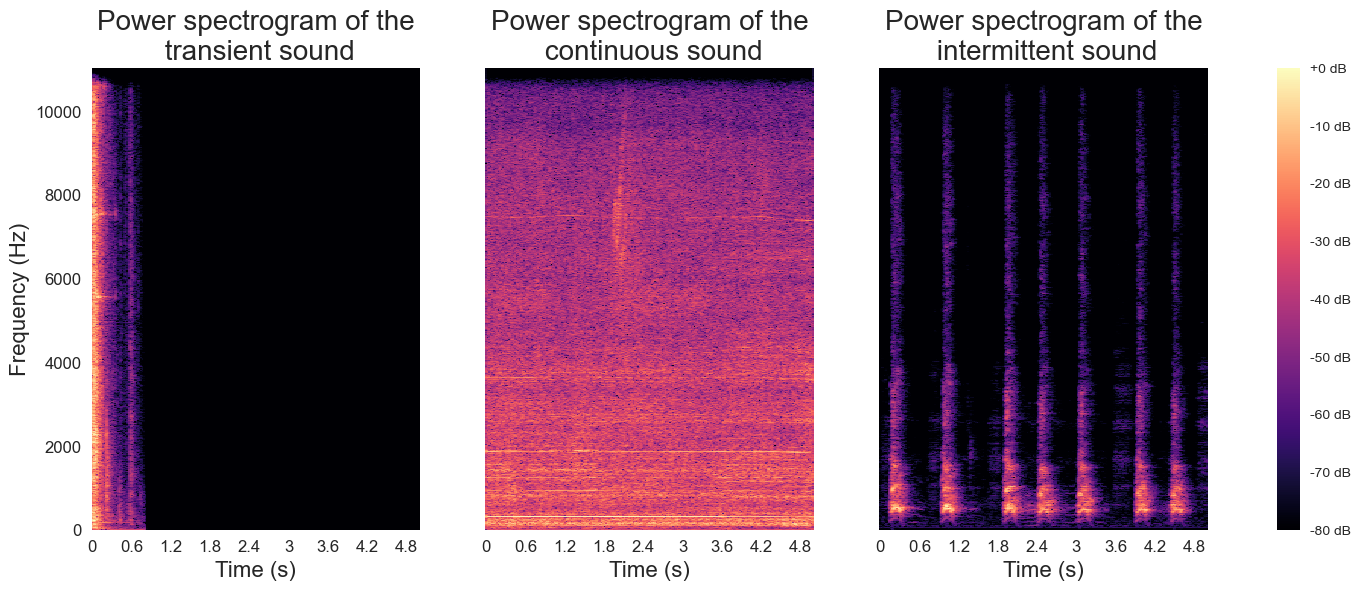
\includegraphics[width=\columnwidth]{Three_types_of_sound.png}}
  \caption{Power spectrogram of a transient, a continous and an intermittent sound.}
  \label{fig:power_spectrograms_3_sounds}
\end{figure}

According to what is reported on the paper in which the ESC-50 dataset is presented \cite{piczak2015dataset}, we higlight how some sounds are more difficult to classify than others,
such as the sounds of a washing machine, an helicopter, or an engine due to their similar spectrograms. If we look to Fig.~\ref{fig:Ambiguous_sounds}, we can see how the three spectrograms
are extremely similar.

\begin{figure}[ht]
  \centering
  \centerline{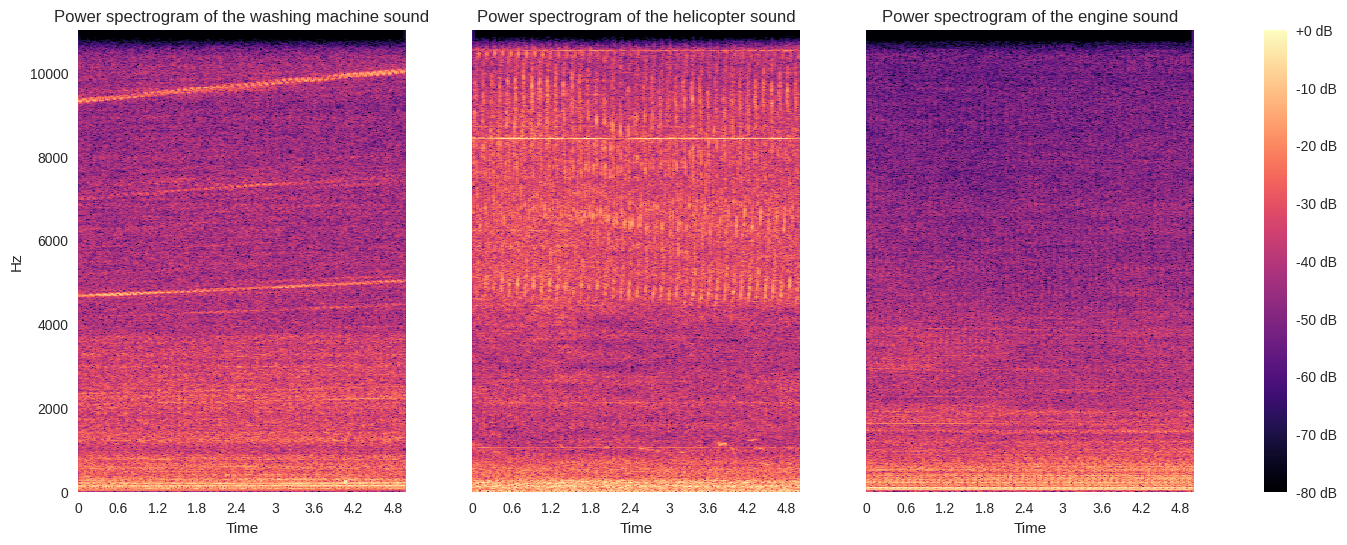
\includegraphics[width=\columnwidth]{Ambiguous_sounds.png}}
  \caption{Power spectrogram of the sound produced by a washing machine, an helicopter and an engine.}
  \label{fig:Ambiguous_sounds}
\end{figure}

This misclassification happens not only for machines, but for humans too. This will be taken into account in the results section, where we will see how the model performs on different classes of sounds.

It is also important to note that, even though we consider the same class, the variability of the sounds is very high, as we can see by comparing the spectrograms of three different
samples of the \textit{dog barking} class. As we can see in Fig.~\ref{fig:Dog_barking}, the three spectrograms are very different from each other. According to the classification defined at the beginngin,
the first one can be considered an impulsive sound, the second one a continuous sound, and the third one an intermittent sound. This means that, given the nature of the sound in this class,
the onset information is not so useful.

\begin{figure}[ht]
  \centering
  \centerline{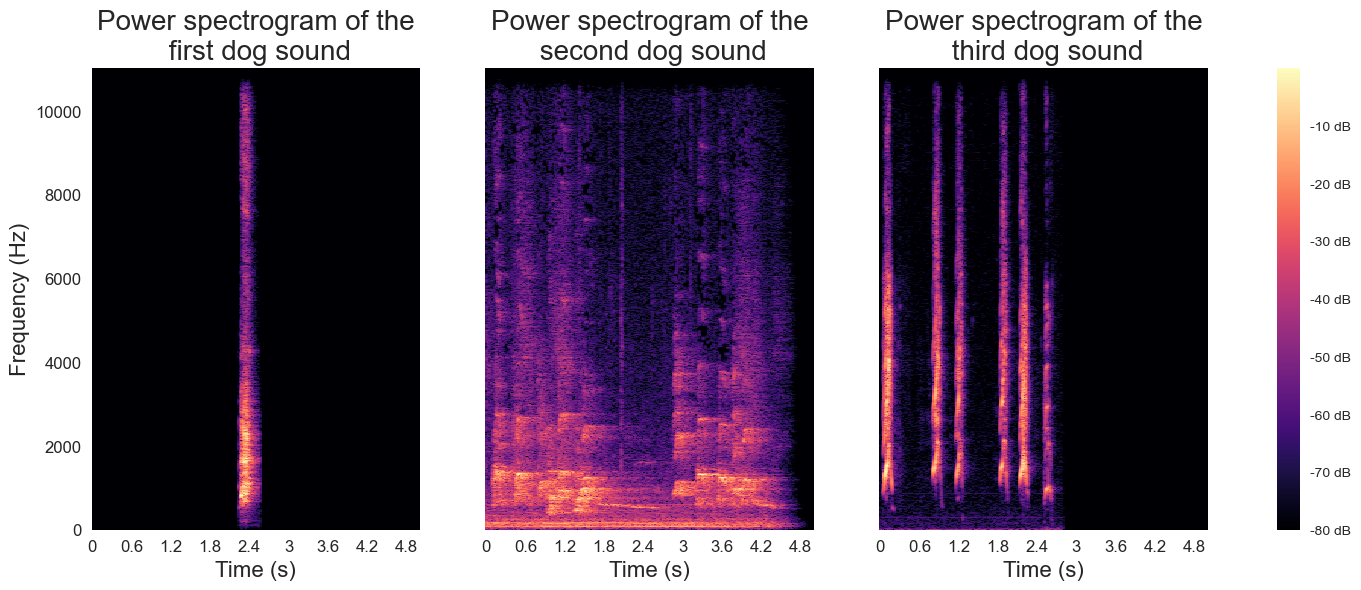
\includegraphics[width=\columnwidth]{dog_barking.png}}
  \caption{Power spectrogram of three different sounds belonging to the same \textit{dog barking} class.}
  \label{fig:Dog_barking}
\end{figure}

Furthermore, we underline how some of the ambiental sounds, like the one of the wind, have no univoque structure: by breaking down their
spectrograms in their harmonic and percussive components as it is done in Fig.~\ref{fig:Dog_barking}, it is evident that the difference
it is not so clear since the two plots are almost equal.

\begin{figure}[ht]
  \centering
  \centerline{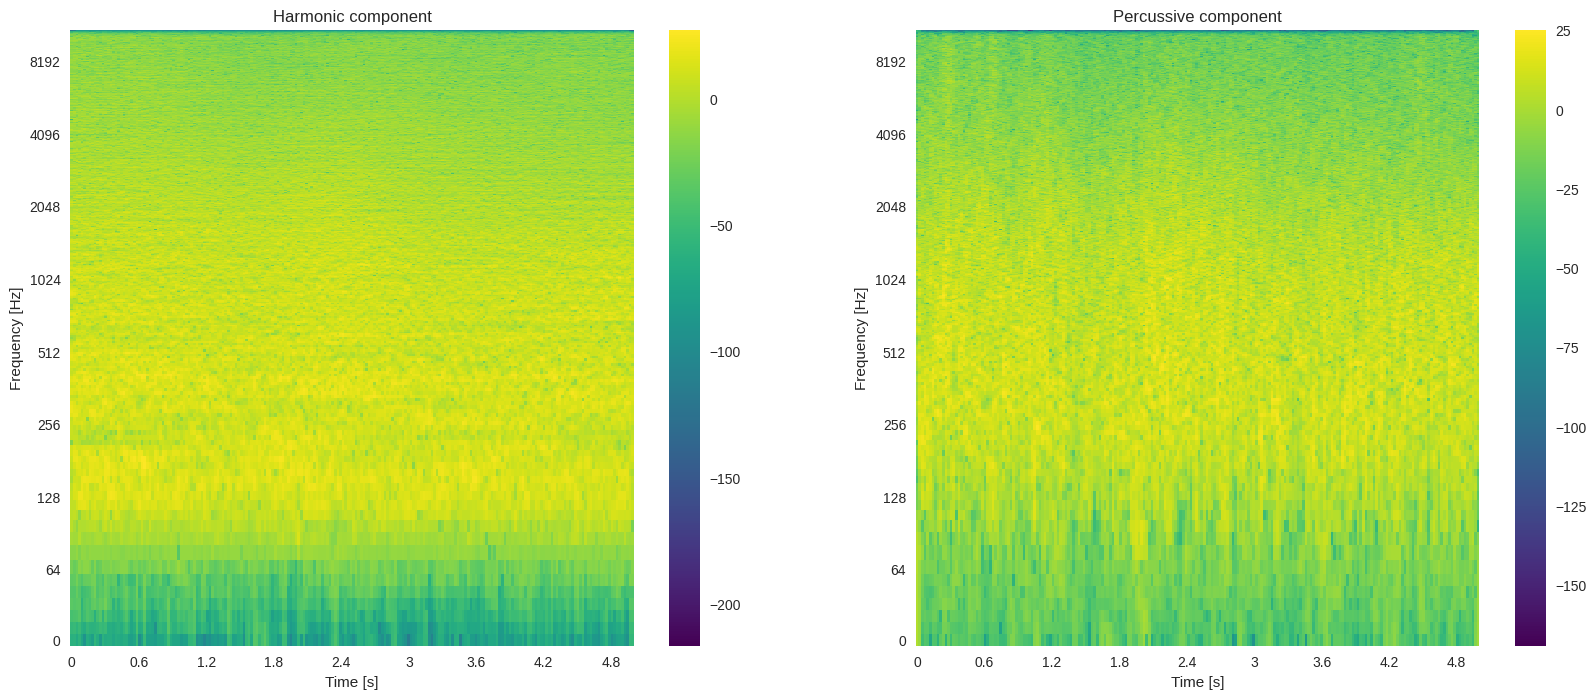
\includegraphics[width=\columnwidth]{Harmonic_Percussive_Wind.png}}
  \caption{Harmonic and percussive decomposition of the wind blowing sound.}
  \label{fig:Harmonic_Percussive_Wind}
\end{figure}

This fast analysis of the dataset has been done to understand the limitations of the model and the difficulties that it could encounter during the training phase.

A part of the dataset, 200 elements (10\% of the total), has been separated for testing. The remaining samples have been splitted according to the stratifiedkfold module of sklearn \cite{scikit-learn_stratifiedkfold} in a training and a validation set.

Drawing inspiration by the Salamon and Bello paper \cite{salamon2017deep}, five different techniques have been implemented to process the training set:
\begin{itemize}
    \item \textbf{Time Stretching (TS)}: the audio signal is stretched or compressed in time by a random factor within a specified range. A last boolean parameter crop the processed audio to the original length, so that the model can be trained on the same length of the original audio.
    \item \textbf{Pitch Shifting (PS)}: the audio signal is shifted in pitch by a random factor within a specified range. [togliere activation probability]
    \item \textbf{Background Noise (BN)}: a Gaussian noise is added to the audio signal with a specified SNR range.
    \item \textbf{Dynamic Range Compression (DRC)}: the dynamic range of the audio signal is compressed from a certain threshold with a specified ratio, attack time, and release time. [Aggiungere che è fatto con la funzione di spotify]
    \item \textbf{Convolution with Impulse Responses (CIR)}: the audio signal is convolved with the \textit{MIT Acoustical Reverberation Scene Statistics Survey} dataset of impulse response \cite{traer2016statistics} to simulate different acoustic environments.
\end{itemize}

[Ce le mettiamo le immagini?]

For all the results presented in this paper, the training dataset has been preprocessed using the following parameters:
\begin{itemize}
    \item TS: factor between 0.8 and 1.25 with an activation probability of 1
    \item PS: factor between -5 and 5 semitones and an activation probability of 1
    \item BN: SNR between 5 and 40 dB, activation probability of 1
    \item DRC: threshold of -20 dB, ratio of 4:1, attack time of 10 ms, release time of 100 ms
    \item CIR: activation probability of 1
\end{itemize}


\subsection{Evaluation metrics}
\label{sec:metrics}
The evaluation of the sound event classification system is performed using several metrics to assess its performance.
Firstly, the test accuracy, the classification reports and the confusion matrix are computed to evaluate the overall performance of the model.




\section{Results}
\label{sec:results}

Ci vanno messi tutti i risultati du quello che abbiamo fatto sul dataset: possiamo così giustificare gli errori di alcune classificazioni.
\textit{La luna vide dal cielo}
\\\textit{Rosita baciar Manuelo}
\\\textit{Con tanto languor, con tanto ardor}
\\\textit{Che s'ammantò d'un velo}

\section{ACKNOWLEDGMENT}
\label{sec:ack}


This work was supported by the Politecnico di Milano,
within the framework of the Selected Topics in Music and Acoustic Engineering Course 2025.
A special thanks goes to the course instructor, Prof. JULIO JOSÉ CARABIAS ORTI, for being
one of the brightest stars in the sky of artificial intelligence.
Last but not least, we would like to thank our wallet: without those 24 euros, we would not have been able to run anything.
Thank you for your support, we are grateful for your generosity.
Grazie a tutt coloro che ci hanno supportato e sopportato.
% -------------------------------------------------------------------------
% Either list references using the bibliography style file IEEEtran.bst
\bibliographystyle{IEEEtran}
\bibliography{refs21}


\end{sloppy}
\end{document}
